% !TeX spellcheck = de_DE
% \documentclass{CPS-Beamer}
\documentclass[aspectratio=169]{CPS-Beamer}
% \documentclass[plain]{CPS-Beamer}

\mode<presentation>

\usepackage[ngerman]{babel}
\usepackage[T1]{fontenc}
\usepackage[utf8]{inputenc}
\title{Bootprocess E310-G000}
\subtitle{SiFive - HiFive1 Board}

\author[Pieper]{Pascal Pieper \\
{\tiny Pascal.Pieper@dfki.de}}
\institute[DFKI CPS]{DFKI GmbH, Cyber-Physical Systems \\ www.dfki.de/cps}

%\date[ISPN '80]{27th International Symposium on Prime Numbers, --280}

\begin{document}

\maketitle
\section{Introduction}
\begin{frame}[plain]
\begin{figure}
	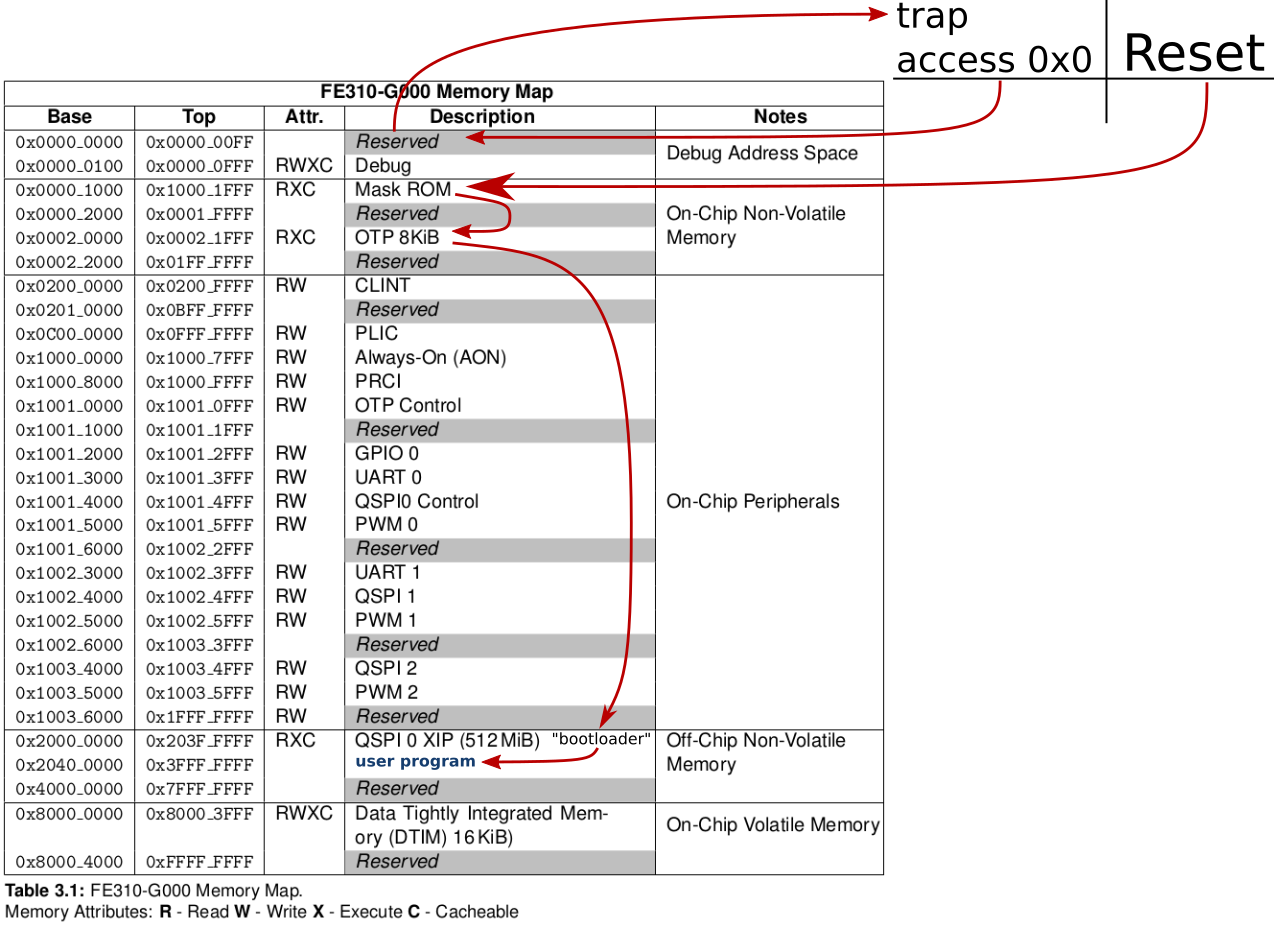
\includegraphics[height=.95\textheight]{MemoryMap_ablauf.png}
	\caption{Modified, from FE310-G000 Manual}
\end{figure}
\end{frame}

\section{Detail}
\begin{frame}{Details}
	\begin{block}{Reset Path}
		\begin{itemize}
			\item Initial program counter at \texttt{0x1000} (MROM)
			\item Mask ROM contains single instruction: Jump to \texttt{0x2\_0000} (OTP)
			\item One Time Programmable Memory jumps to \texttt{0x2000\_0000} (QSPI)
			\item "bootloader" on Flash initializes CPU and jumps to \texttt{0x2040\_0000} (QSPI)
			\item User defined program starts
		\end{itemize}
	\end{block}
\end{frame}

\begin{frame}{Details}
	\begin{block}{Invalid Access (e.g. nullpointer dereference)}
		\begin{itemize}
			\item If trap vector is still default (\texttt{0x0}), a null instruction (\texttt{0x0000\_0000}) is fetched
			\item Trap vector is called again, looping endlessly
			\item ... until reset or \textit{debugger} interrupt
			\item Debug interrupt handler is wired to debug ROM (\texttt{0x0400}) which calls debug RAM (\texttt{0x0800})
			\item Debug RAM may load programs from an \textit{openocd}-session via debug peripheral to "userspace" (\texttt{0x2040\_0000})
			\item Debug RAM finally jumps to user program
		\end{itemize}
	\end{block}
\end{frame}

\section{Special Memory Regions}
\begin{frame}{Special Memory Regions\\~\\OTP (One Time Programmable Memory)}
	\begin{block}{Contains:}
		\begin{itemize}
			\item Trim settings for Internal Oscillator (HFROSC)
			\item Configuration string for chip information
			\item (Jump to flash bootloader)
		\end{itemize}
	\end{block}
\end{frame}


\section{Special Memory Regions}
\begin{frame}{Special Memory Regions\\~\\Bootloader}
	\begin{block}{Scenario}
		\begin{itemize}
			\item User Program modifies system clock and "breaks" the execution
			\item Debugger peripheral is also dependent on clock
			\item[$\rightarrow$] Device can't be programmed\\(too little time between reset and execution of "malicious" user program)
		\end{itemize}
	\end{block}
	\begin{block}{Solution}
	\begin{itemize}
		\item "bootloader" gets executed first and checks for wakeup reason
		\item If (manually) reset twice inside booloader, it stops execution (spinlock)
		\item[$\rightarrow$] user can upload new (hopefully better) program via debugger
	\end{itemize}
\end{block}
\end{frame}



\end{document}
